\section{Robot Results}
Much of this work is motivated by our experiences with the ROS navigation stack \cite{marder:office}. Initially, it did not have a way to directly input non-lethal obstacles. One could only input lethal obstacles, and have a small buffer of non-lethal obstacles surround it, which made it difficult to model people's personal space. As a result, we created a branch of the navigation stack that allowed for arbitrary changes to be made to the costmap. Typical parameters for the global costmap involve a grid resolution of 5 centimeters and a planning constant of $P=50$. Amplitudes can range from $[0, 254]$ and variance was typically set between $0$ and $2$. The robot was command to move from $(-3[m], 0)$ to $(+3[m], 0)$. The costmap data is then passed into a modified wavefront planner that performs interpolated gradient descent to determine a smooth path, one not constrained by the shape of the grid. 

The biggest question that these experiments intended to figure out was whether the same relations between parameters that we observed in the simple 4-connected grid would hold up in this less restricted environment. As seen in Figure \ref{fig:realdata}, the same principles apply. Since costmaps and the discretized paths they produce are all approximations of the same continuous space, it is logical that the different grid connectivities would have similar results, however, it is nice to have the technical confirmation to back up the ideas. Not only is the solution more general, but it has the added benefit that the resulting smoother paths are more legible to people observing the robot. 


\newcommand{\rrrr}{.3}
\begin{figure*}[b]
\centering
\subfloat[$A=250$, $\sigma=0.15$]{
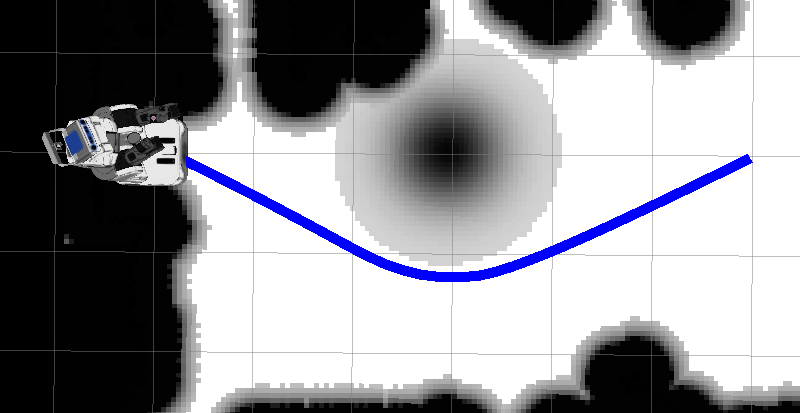
\includegraphics[width=\rrrr\textwidth]{graphix/250-p15.png}
\label{fig:d1}}
\subfloat[$A=250$, $\sigma=0.30$]{
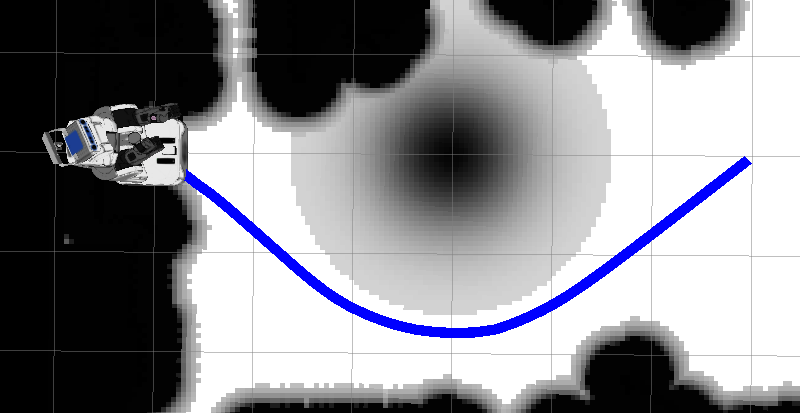
\includegraphics[width=\rrrr\textwidth]{graphix/250-p3.png}
\label{fig:d2}}
\subfloat[$A=250$, $\sigma=0.60$]{
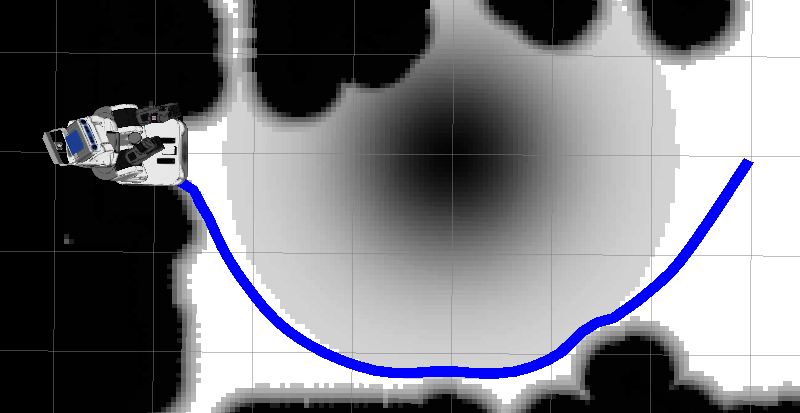
\includegraphics[width=\rrrr\textwidth]{graphix/250-p6.png}
\label{fig:d3}}\\
\subfloat[$A=250$, $\sigma=0.90$]{
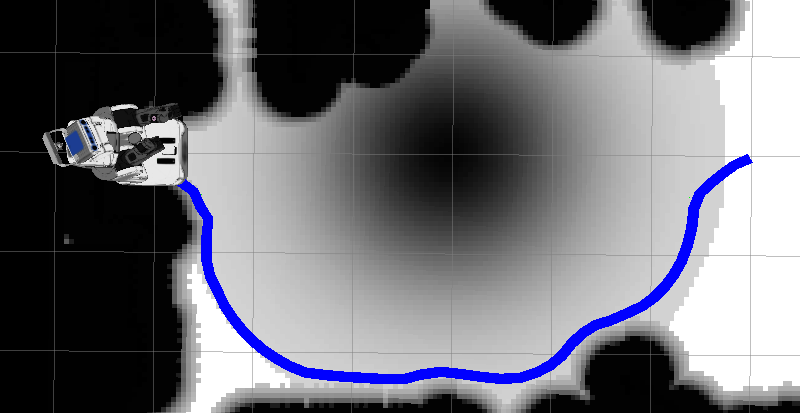
\includegraphics[width=\rrrr\textwidth]{graphix/250-p9.png}
\label{fig:d4}}
\subfloat[$A=250$, $\sigma=1.20$]{
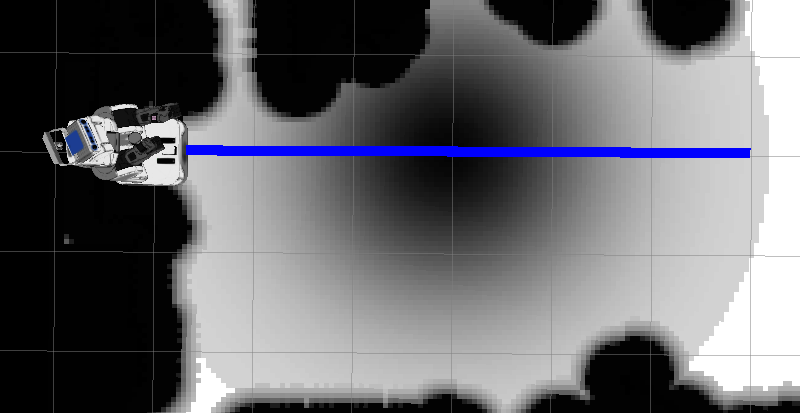
\includegraphics[width=\rrrr\textwidth]{graphix/250-1p2.png}
\label{fig:d5}}
\subfloat[$A=150$, $\sigma=1.20$]{
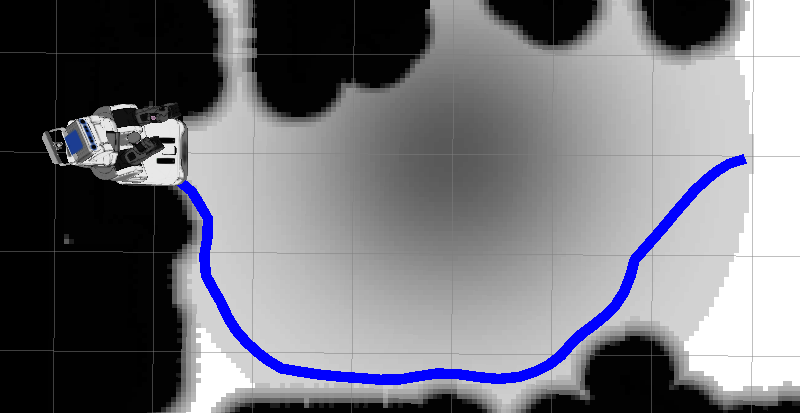
\includegraphics[width=\rrrr\textwidth]{graphix/150-1p2.png}
\label{fig:d6}}
\caption{Real plans generated by the ROS Navigation Stack - As the variance increases (a)-(d), the path gets further from the obstacle. However, in (e) when the variance is over 1, the path reverts to straight through. However, by setting the amplitude to a smaller number, while keeping the variance constant, (f), we can again derive a not straight plot.  }
\label{fig:realdata}
\end{figure*}

